\documentclass[russian,utf8,12pt]{eskdtext}
\usepackage[numbertop, numbercenter]{eskdplain}

% - Подключаем шрифты из пакета scalable-cyrfonts-tex
\usepackage{cyrtimes}

% - Отступ красной строки
\setlength{\parindent}{1.25cm}

% - Убирает точку в списке литературы
\makeatletter
\def\@biblabel#1{#1 }

% - Точки для всех пунктов в оглавлении
\renewcommand*{\l@section}{\@dottedtocline{1}{1.5em}{2.3em}}
\renewcommand*{\l@subsection}{\@dottedtocline{1}{1.5em}{2.3em}}
\renewcommand*{\l@subsubsection}{\@dottedtocline{1}{1.5em}{2.3em}}

% - Для переопределения списков
\renewcommand{\theenumi}{\arabic{enumi}}
\renewcommand{\labelenumi}{\theenumi)}
\makeatother

\usepackage{enumitem}
\setlist{nolistsep, itemsep=0.3cm,parsep=0pt}

% - ГОСТ списка литературы
\bibliographystyle{utf8gost705u}

% - Верикальные отступы заголовков 
\ESKDsectSkip{section}{1em}{1em}
\ESKDsectSkip{subsection}{1em}{1em}
\ESKDsectSkip{subsubsection}{1em}{1em}

% - Изменение заголовков
\usepackage{titlesec}
\titleformat{\section}{\centering\normalfont\normalsize}{\thesection}{1.0em}{}
\titleformat{\subsection}{\centering\normalfont\normalsize}{\thesubsection}{1.0em}{}
\titleformat{\subsubsection}{\centering\normalfont\normalsize}{\thesubsubsection}{1.0em}{}
\titleformat{\paragraph}{\centering\normalsize}{\theparagraph}{1.0em}{}

% - Оставим место под ТЗ 
%\setcounter{page}{4}

% - Для больших таблиц
\usepackage{longtable}
\usepackage{tabularx}
\renewcommand{\thetable}{\thesection.\arabic{table}}

% - Используем графику в документе
\usepackage{graphicx}
\graphicspath{{images/}}
\renewcommand{\thefigure}{\thesection.\arabic{figure}}

% - Счётчики
\usepackage{eskdtotal}

% - Выравнивание по ширине
\sloppy

% - Разрешить перенос двух последних букв слова
\righthyphenmin=2

\RequirePackage{enumitem}
\renewcommand{\alph}[1]{\asbuk{#1}}
\setlist{nolistsep}
\setitemize[1]{label=--, fullwidth, itemindent=\parindent, 
  listparindent=\parindent}% для дефисного списка
\setenumerate[1]{label=\arabic*), fullwidth, itemindent=\parindent, 
  listparindent=\parindent}% для нумерованного списка
\setenumerate[2]{label=\alph*), fullwidth, itemindent=\parindent, 
  listparindent=\parindent, leftmargin=\parindent}% для списка 2-ой ступени, который будет нумероваться а), б) и т.д.

\usepackage{listings}  
\lstset{basicstyle=\ttfamily\small}

\begin{document}

\section{Документирование плагинов}

На данный момент основной репозиторий находится на ресурсе GitHub. Данный ресурс использует язык разметки MarkDown (подробнее в разделе ~\ref{sec:markdown}) и автоматически добавляет файл "Readme.md" к описанию программного модуля, если этот файл присутствует. В связи с этим было решено создать документацию плагинов, используя MarkDown. Документация должна включать в себя:

\begin{enumerate}
  \item Название плагина;
  \item Версию плагина;
  \item Автора плагина;
  \item Описание плагина;
  \item Требуемую операционную систему;
  \item Версию ПО, с которым этот плагин работает;
  \item Основные методы плагина с описанием входов и выходов.
\end{enumerate}

Результат разработанной документации можно наблюдать на странице плагина в репозитории ~\ref{bok_1:bok_1}

\begin{figure}[!ht]
\center{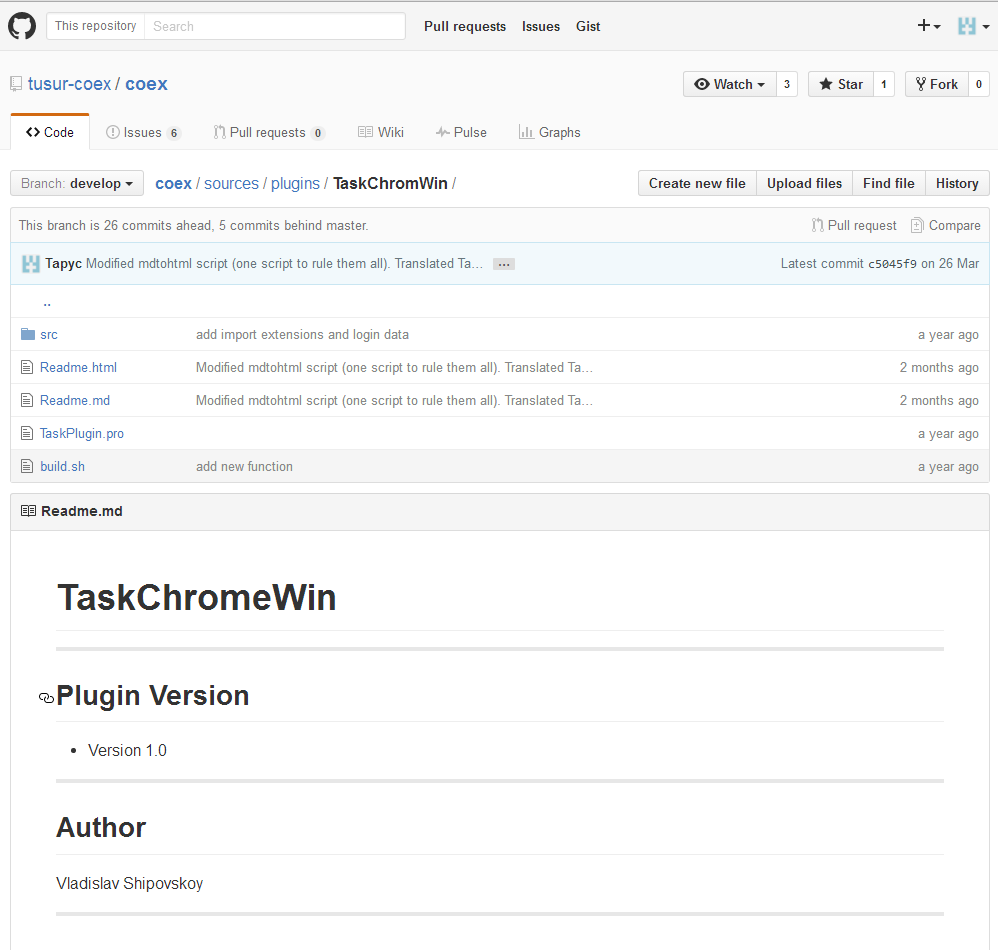
\includegraphics[width=1\linewidth]{bok_1}}
\caption{ Документация в веб-интерфейсе репозитория }
\label{bok_1:bok_1}
\end{figure}

Поскольку проект "coex" имеет свою собственную веб-страницу, данную документацию также необходимо преобразовать в формат HTML, чтобы затем добавить на веб-страницу проекта. Для преобразования был разработан небольшой скрипт на языке Python (приложение ~\ref{apx:mdtohtml}). На рисунке ~\ref{bok_2:bok_2} можно наблюдать ту же документацию, но в формате HTML.

\begin{figure}[!ht]
\center{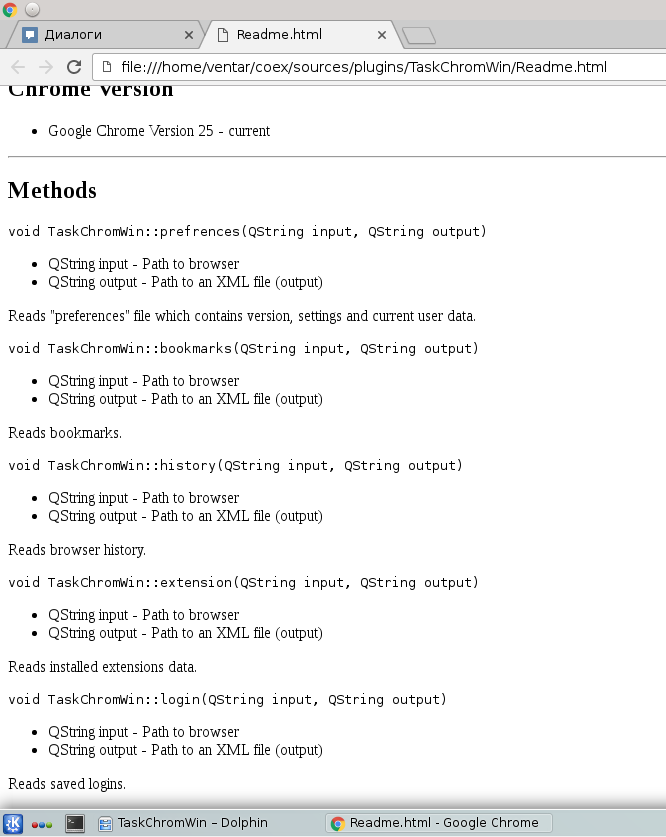
\includegraphics[width=1\linewidth]{bok_2}}
\caption{ Документация в формате HTML }
\label{bok_2:bok_2}
\end{figure}

\section{Разработка и внедрение копии жесткого диска}

Поскольку большое количество плагинов "coex" обращается к жесткому диску для поиска тех или иных файлов, что в свою очередь создает серьезную нагрузку на него, то было решено модифицировать архитектуру проекта с целью хранения копии информации о жестком диске. Данную информацию решено было хранить как поле объекта "config", к которому будут обращаться остальные плагины. Поле представляет из себя класс "Hdd" с атрибутом типа QList<QDir> (приложение ~\ref{apx:hddclass}). Данный тип был выбран, поскольку он позволяет хранить данные о всех директориях и файлах внутри них, а также предоставляет удобные интерфейсы для доступа к ним. Методы класса "Hdd":

\begin{enumerate}
  \item Hdd::Hdd(QString path)
  \item Hdd::~Hdd()
  \item QFileInfoList getFiles(QStringList wildcardlist);
  \item QFileInfoList getFiles(QString wildcard).
\end{enumerate}

Метод "Hdd::Hdd(QString path)" является конструктором класса. Переменная "path", подаваемая на вход метода является путем до начальной папки. Конструктор с помощью экземпляра класса "QDirIterator" посещает каждую папку в начальной папке и сохраняет данные о ней в переменную типа "QDir", после чего добавляет эту переменную к массиву "QList<QDir>", и наконец сохраняет полученный массив как поле класса. Алгоритм конструктора можно увидеть на рисунках ~\ref{bok_6:bok_6} и ~\ref{bok_7:bok_7}.

\begin{figure}[!ht]
\center{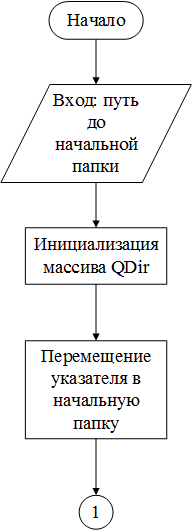
\includegraphics[width=1\linewidth]{bok_6}}
\caption{ Алгоритм конструктора класса "Hdd" }
\label{bok_6:bok_6}
\end{figure}

\begin{figure}[!ht]
\center{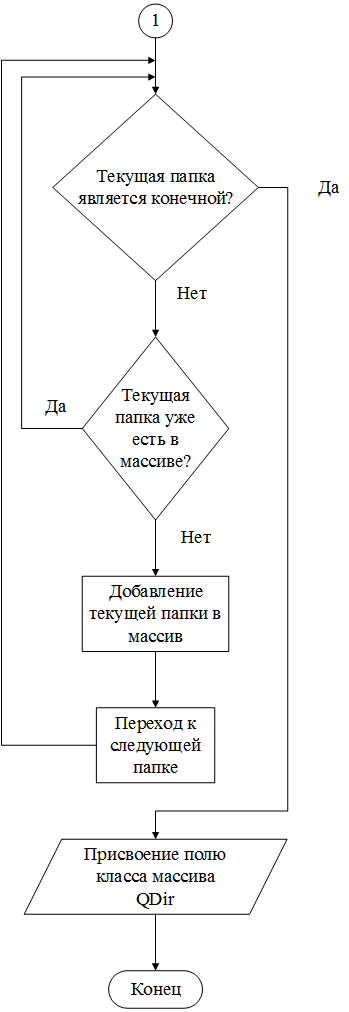
\includegraphics[width=1\linewidth]{bok_7}}
\caption{ Продолжение алгоритма конструктора класса "Hdd" }
\label{bok_7:bok_7}
\end{figure}

Метод "Hdd::~Hdd()" является деструктором класса.
Метод "QFileInfoList getFiles(QStringList wildcardlist)" возвращает объект "QFileInfoList" для всех файлов, которые соответствуют заданному массиву масок "wildcardlist". Алгоритм метода можно увидеть на рисунке ~\ref{bok_9:bok_9}.

\begin{figure}[!ht]
\center{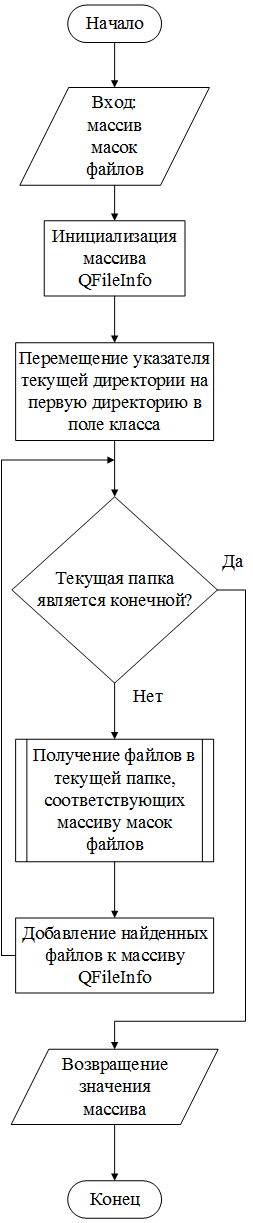
\includegraphics[width=1\linewidth]{bok_9}}
\caption{ Продолжение алгоритма конструктора класса "Hdd" }
\label{bok_9:bok_9}
\end{figure}

Метод "QFileInfoList getFiles(QString wildcard)" выполняет ту же функцию, что и прошлый метод. Он является перегрузкой прошлого метода и принимает на вход одну маску вместо массива. Алгоритм метода можно увидеть на рисунке ~\ref{bok_8:bok_8}.

\begin{figure}[!ht]
\center{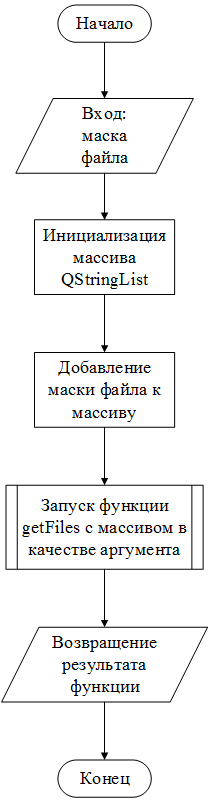
\includegraphics[width=1\linewidth]{bok_8}}
\caption{ Продолжение алгоритма конструктора класса "Hdd" }
\label{bok_8:bok_8}
\end{figure}

После разработки архитектуры класса, он был внедрен в "скелет" проекта. Класс конструируется перед работой плагинов, но после определения операционной системы.

\begin{figure}[!ht]
\center{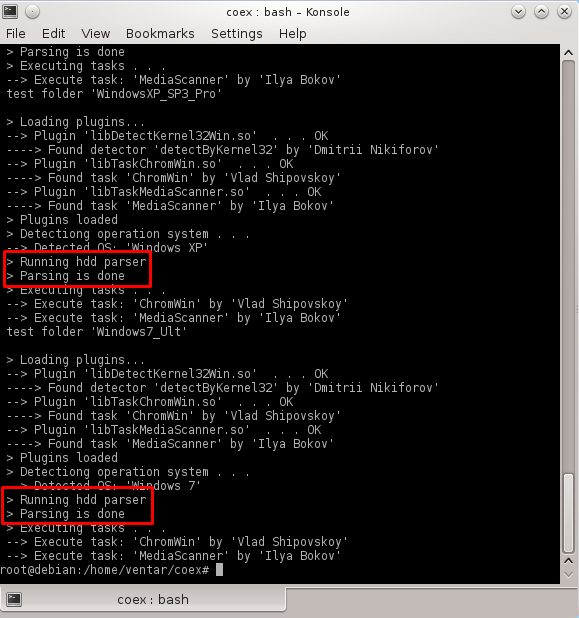
\includegraphics[width=1\linewidth]{bok_3}}
\caption{ Работа класса "Hdd" при запуске "coex" }
\label{bok_3:bok_3}
\end{figure}

Далее необходимо было изменить плагины, таким образом, чтобы они обращались к сохраненной копии диска вместо самого диска. Таким образом были изменены два плагина - "TaskMediaScanner" и "TaskChromeWin".
Теперь перед нами стояла задача сравнить нагрузку диска до и после внедрения класса "Hdd". Поскольку нами использовался удаленный репозиторий и система контроля версий git, то это не составило проблемы по причине того, что разработка класса велась в отдельной "ветке".
Было решено с помощью утилиты iotop замерить использование жесткого диска (в КБ/с) несколько раз до и после введения нового плагина и отфильтровать полученные результаты, чтобы учитывать исключительно нагрузку, создаваемую программой "coex". Для этого был разработан мультипоточный скрипт на языке Python, запускающий отдельно утилиту "iotop" и "coex" и фильтрующий результаты, сохраняемые утилитой "iotop" (приложение ~\ref{apx:diskusage}):

\begin{figure}[!ht]
\center{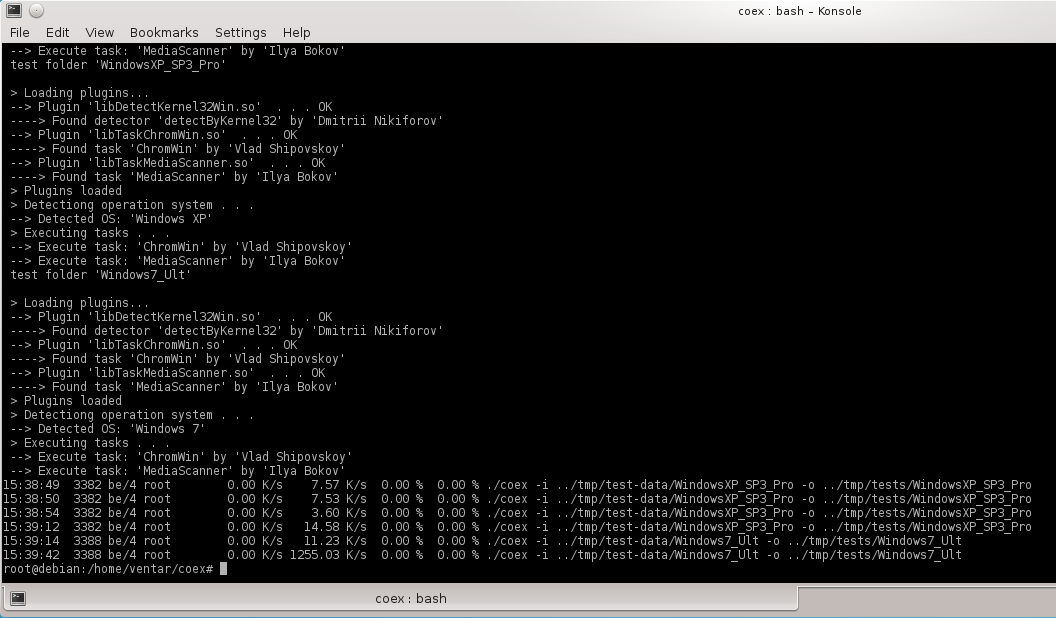
\includegraphics[width=1\linewidth]{bok_4}}
\caption{ Результат работы скрипта }
\label{bok_4:bok_4}
\end{figure}

Далее результаты были обработаны, и на основании их был построен график, показывающий нагрузку на жесткий диск до и после внедрения класса "Hdd". Было решено оставить по 10 итераций на каждое измерение, поскольку после этого количества разница между итерациями была минимальна и уже прослеживалась значимая разница между измерениями.

\begin{figure}[!ht]
\center{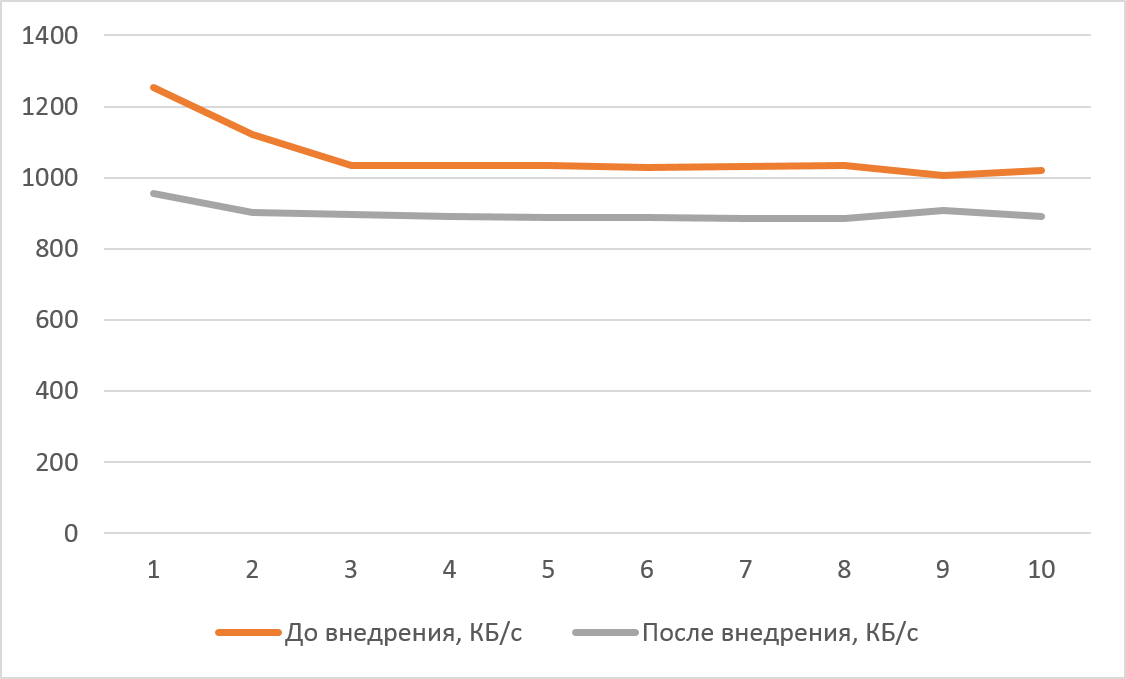
\includegraphics[width=1\linewidth]{bok_5}}
\caption{ Сравнение нагрузки на жесткий диск до и после изменения архитектуры }
\label{bok_5:bok_5}
\end{figure}

Из графика видно, что даже при изменении всего двух плагинов для использования новой архитектуры нагрузка на диск заметно снизилась. Так как на данный момент в проекте "coex" имеется 17 рабочих плагинов, преобразование каждого из них должно сильно сказаться на нагрузке жесткого диска в лучшую сторону.

\clearpage
\end{document}
